\chapter{Kế hoạch thực hiện đồ án tốt nghiệp}

\section{Mục tiêu tổng thể}
Đồ án tốt nghiệp nhằm hoàn thiện và triển khai hệ thống Trục Tích Hợp Dữ Liệu cho Trường Đại Học dựa trên nền tảng kiến trúc API-led Connectivity, kế thừa kết quả thiết kế kiến trúc từ đồ án chuyên ngành, tiến tới hiện thực hóa hệ thống ở mức độ thực tế (production-like).

Mục tiêu chính:

\begin{itemize}
    \item Xây dựng trục tích hợp dữ liệu hoạt động theo mô hình One-way Integration Hub
    \item Đảm bảo tính nhất quán, bảo mật và khả năng mở rộng

    \item Hoàn thiện tài liệu kỹ thuật, triển khai, kiểm thử và đánh giá hệ thống
\end{itemize}

\section{Phân chia giai đoạn thực hiện}

Dự án được dự định chia thành 6 giai đoạn chính, triển khai liên tục từ tháng 01/2026 đến tháng 05/2026.

\begin{figure}[htbp]
  \centering
  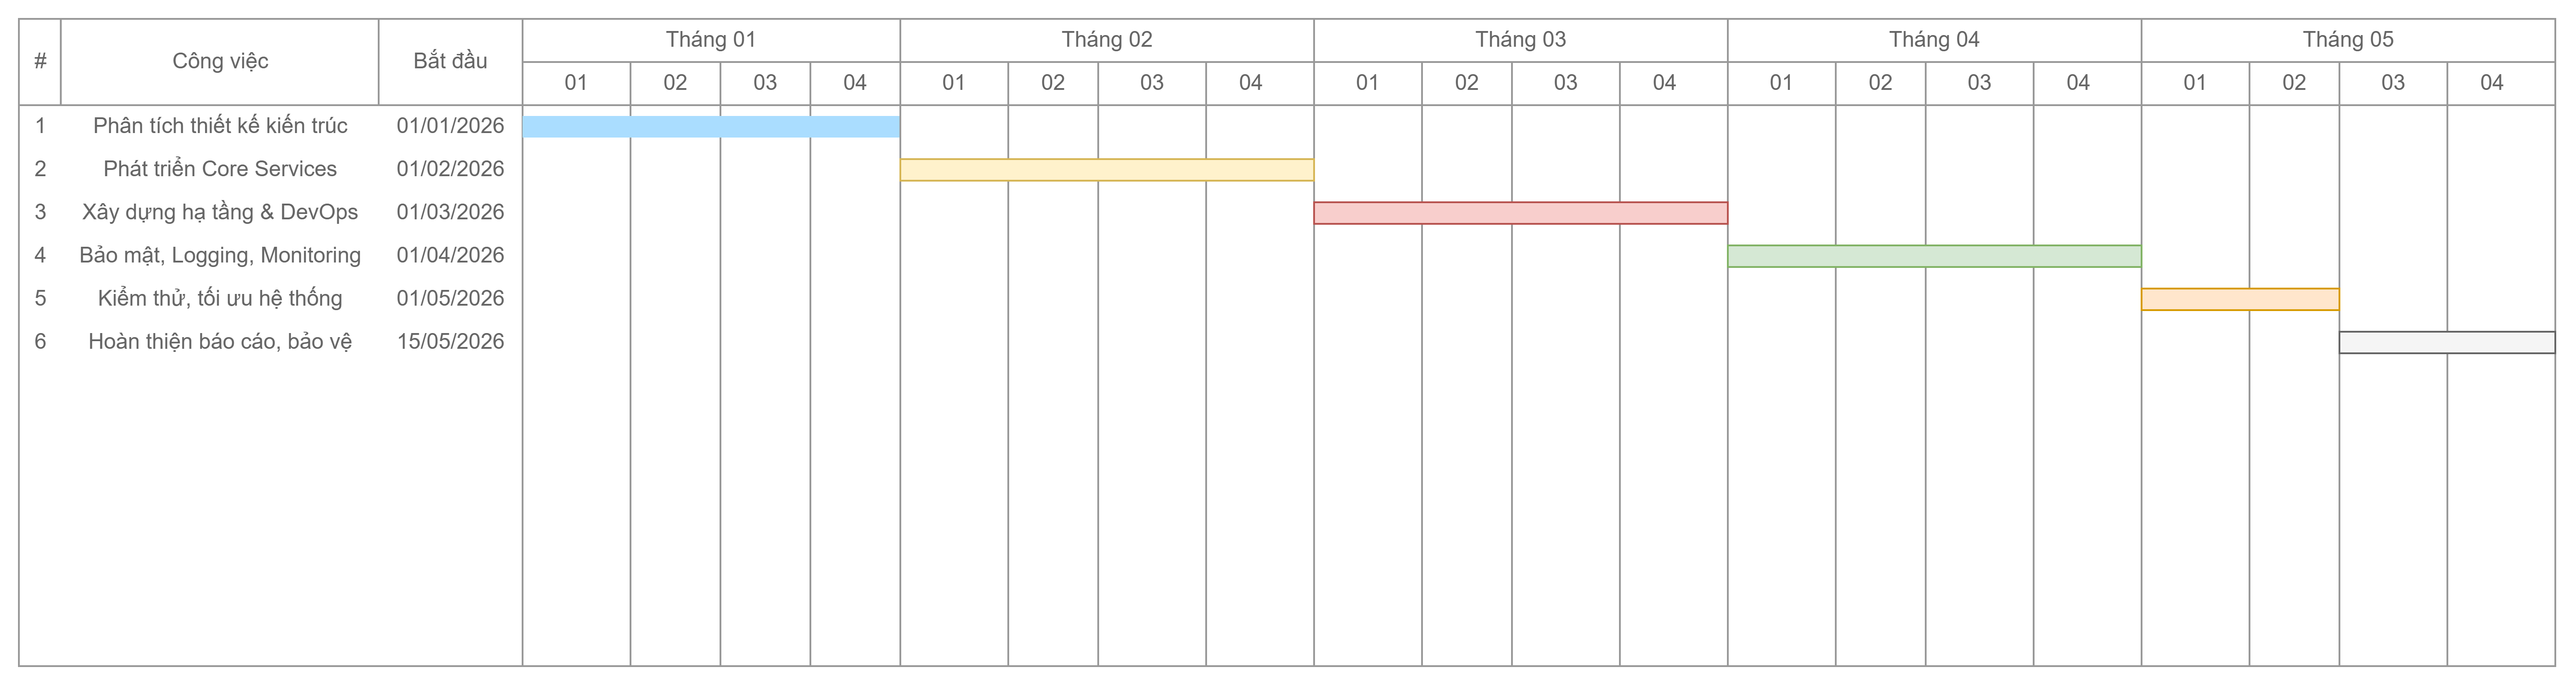
\includegraphics[width=0.6\textwidth]{graphics/gantt.png}
  \caption{Biểu đồ Gantt cho kế hoạch thực hiện đồ án}
\end{figure}


\subsection{Giai đoạn 1: Phân tích \& Hoàn thiện thiết kế (01/2026)}

\textbf{Mục tiêu}: Rà soát toàn bộ kiến trúc đã đề xuất trong đồ án chuyên . Hoàn thiện thiết kế chi tiết cho đồ án tốt . Chuẩn hóa yêu cầu chức năng và phi chức năng

\textbf{Công việc thực hiện:}
\begin{itemize}
    \item Phân tích lại yêu cầu hệ thống trục tích hợp
    \item Hoàn thiện: Deployment Architecture; Security Architecture (4 layer security); Data Flow Diagram; API-led Connectivity Model
    \item Thiết kế: Data Model trung tâm (PostgreSQL); API Contracts (OpenAPI); Quy trình backup, logging, monitoring
    \item  Lập kế hoạch triển khai chi tiết cho các giai đoạn tiếp theo
\end{itemize}

\textbf{Phân công}

\begin{itemize}
    \item Tuấn: Thiết kế kiến trúc tổng thể; Security Architecture; API Gateway \& Auth Flow
    \item Huy: Data Model \& Database Design; Backup, Data Governance; Observability \& Logging Design
\end{itemize}

\textbf{Sản phẩm đầu ra}

\begin{itemize}
    \item Tài liệu thiết kế kiến trúc hoàn chỉnh
    \item Sơ đồ hệ thống (PNG)
    \item Chương Kiến trúc \& Thiết kế trong báo cáo
\end{itemize}

\subsection{Giai đoạn 2: Phát triển Core Services (02/2026)}
\textbf{Mục tiêu:} Hiện thực hóa trục tích hợp dữ liệu; Xây dựng các API chính của hệ thống

\textbf{Công việc thực hiện}

\begin{itemize}
    \item Phát triển: Data Integration Server (ingest data từ SIS/LMS giả lập); Data Sharing Server (API truy vấn dữ liệu)
    \item Xây dựng: API chuẩn hóa dữ liệu; Validation \& Mapping
    \item Áp dụng: JWT Authentication; Role/Permission-based Authorization

    \item Ghi log nghiệp vụ (Security Logging)
\end{itemize}

\textbf{Phân công}\begin{itemize}
    \item Tuấn: Auth \& Authorization; API Gateway Integration; Security Middleware
    \item Huy: Data Processing Logic; Data Validation; Database Interaction
\end{itemize}

\textbf{Sản phẩm đầu ra}

\begin{itemize}
    \item Trục tích hợp dữ liệu hoạt động
    \item API truy vấn dữ liệu ổn định
    \item Swagger/OpenAPI Documentation
\end{itemize}

\subsection{Giai đoạn 3: Xây dựng hạ tầng \& DevOps (03/2026)}

\textbf{Mục tiêu:} Chuẩn bị môi trường triển khai và pipeline DevOps; Đảm bảo hệ thống có thể build – deploy – rollback

\textbf{Công việc thực hiện}

\begin{itemize}
    \item Thiết lập:Git repository (GitHub/GitLab); CI/CD Pipeline
    \item Docker hóa: NestJS Services; Auth Service
    \item Cấu hình: Kong API Gateway; PostgreSQL; MinIO
    \item Thiết lập: Prisma ORM \& Prisma Migrate. Biến môi trường \& Secret Management
    \item  Triển khai pipeline: build image; migrate schema; deploy rolling/canary
\end{itemize}

\textbf{Phân công}

\begin{itemize}
    \item Tuấn: CI/CD Pipeline; Kong Gateway; Auth Service.
    \item Huy: Docker \& PostgreSQL; Prisma \& Migration; MinIO Backup Infrastructure
\end{itemize}

\textbf{Sản phẩm đầu ra}

\begin{itemize}
    \item Pipeline CI/CD hoạt động
    \item Môi trường triển khai hoàn chỉnh
    \item Tài liệu DevOps \& Deployment
\end{itemize}

\subsection{Giai đoạn 4: Hoàn thiện bảo mật, logging \& monitoring (04/2026)}

\textbf{Mục tiêu:} Đảm bảo hệ thống đạt mức bảo mật và giám sát cao; Chuẩn bị cho kiểm thử tổng thể

\textbf{Công việc thực hiện:}

\begin{itemize}
    \item Tích hợp: Filebeat / Logstash; Elasticsearch; Kibana Dashboard
    \item Cấu hình: Alerting; Rate Limiting; Input Validation
    \item Hoàn thiện: Backup \& Restore; RPO/RTO
    \item Kiểm thử bảo mật: JWT; Permission; Rate limiting
\end{itemize}

\textbf{Phân công}

\begin{itemize}
    \item Tuấn: Security Testing; API Gateway Policies
    \item Huy: Logging Pipeline; Monitoring Dashboard; Backup \& Restore Testing
\end{itemize}


\textbf{Sản phẩm đầu ra}
\begin{itemize}
    \item Hệ thống giám sát hoạt động
    \item Dashboard Kibana
    \item Báo cáo bảo mật \& logging
\end{itemize}


\subsection{Giai đoạn 5: Kiểm thử tổng thể \& tối ưu (05/2026 - đầu tháng)}

\textbf{Mục tiêu:} Đánh giá chất lượng hệ thống; Tối ưu hiệu năng và độ ổn định

\textbf{Công việc thực hiện}

\begin{itemize}
    \item Thực hiện: Unit Test; Integration Test; Load Test (giả lập LMS/MyBK)
    \item Đánh giá: Hiệu năng API; Khả năng chịu tải
    \item Tối ưu: Query; Index DB; Cache (nếu cần)
\end{itemize}

\textbf{Sản phẩm đầu ra}

\begin{itemize}
    \item Báo cáo kiểm thử
    \item Biểu đồ đánh giá hiệu năng
    \item Phiên bản hệ thống ổn định
\end{itemize}


\subsection{Giai đoạn 6: Hoàn thiện báo cáo \& bảo vệ (Cuối 05/2026)}

\textbf{Mục tiêu:} Hoàn tất đồ án tốt nghiệp; Chuẩn bị bảo vệ

\textbf{Công việc thực hiện}

\begin{itemize}
    \item Viết và chỉnh sửa: Báo cáo đồ án; Phụ lục kỹ thuật
    \item Chuẩn bị: Slide thuyết trình; Demo hệ thống
    \item Tổng hợp: Kết luận; Hướng phát triển tương lai
\end{itemize}


\textbf{Sản phẩm đầu ra}
\begin{itemize}
    \item Báo cáo hoàn chỉnh
    \item Slide bảo vệ
    \item Hệ thống demo
\end{itemize}

\chapter{Tổng kết đồ án chuyên ngành}

\section{Những điểm đã đạt được}

Trong khuôn khổ đồ án chuyên ngành, nhóm đã tiến hành nghiên cứu, phân tích và đề xuất một giải pháp tổng thể cho bài toán tích hợp dữ liệu trong môi trường trường đại học, nơi tồn tại nhiều hệ thống thông tin độc lập như hệ thống quản lý đào tạo, hệ thống quản lý học tập (LMS), hệ thống nhân sự, tài chính và các cổng thông tin nội bộ. Thông qua quá trình khảo sát thực tế và tham khảo các mô hình tích hợp hiện đại, đồ án đã xác định rõ nhu cầu cấp thiết về một trục tích hợp dữ liệu đóng vai trò trung gian, giúp chuẩn hóa, thu thập và cung cấp dữ liệu một cách nhất quán giữa các hệ thống.

Kết quả nổi bật đầu tiên của đồ án là việc xây dựng được cái nhìn tổng quan và có hệ thống về các mô hình trục tích hợp dữ liệu, bao gồm kiến trúc ESB truyền thống và các kiến trúc hiện đại hơn như API-led Connectivity. Trên cơ sở so sánh ưu, nhược điểm của từng mô hình, đồ án đã đề xuất kiến trúc trục tích hợp dữ liệu dựa trên API-led Connectivity, phù hợp với xu hướng microservices và yêu cầu mở rộng linh hoạt trong môi trường đại học. Kiến trúc đề xuất đã làm rõ vai trò của các thành phần chính như API Gateway, Integration Server, Data Sharing Server, Auth Service và cơ sở dữ liệu trung tâm, cũng như luồng dữ liệu một chiều từ các hệ thống nguồn về trục tích hợp.

Bên cạnh kiến trúc tổng thể, đồ án chuyên ngành cũng đạt được những kết quả quan trọng trong việc thiết kế các khía cạnh kỹ thuật cốt lõi của hệ thống. Cụ thể, nhóm đã đề xuất nền tảng công nghệ phù hợp cho từng thành phần, trong đó NestJS được lựa chọn làm nền tảng backend cho các dịch vụ tích hợp và chia sẻ dữ liệu, PostgreSQL được sử dụng làm cơ sở dữ liệu trung tâm, Kong API Gateway đóng vai trò tuyến phòng thủ và điều phối truy cập, cùng với MinIO cho lưu trữ backup. Ngoài ra, đồ án đã xây dựng được mô hình bảo mật tổng thể nhiều lớp, bao gồm xác thực và phân quyền dựa trên JWT, mã hóa dữ liệu khi truyền và khi lưu trữ, cũng như các cơ chế giám sát, ghi log và cảnh báo nhằm đảm bảo an toàn và khả năng truy vết của hệ thống.

Một đóng góp đáng kể khác của đồ án là việc thiết kế chi tiết các sơ đồ kiến trúc, sơ đồ luồng dữ liệu và sơ đồ triển khai, giúp làm rõ cách thức các thành phần tương tác với nhau trong một hệ thống trục tích hợp hoàn chỉnh. Những sơ đồ này không chỉ hỗ trợ cho việc hiểu rõ giải pháp đề xuất mà còn đóng vai trò là nền tảng quan trọng để hiện thực hóa hệ thống trong giai đoạn đồ án tốt nghiệp tiếp theo. Ngoài ra, đồ án cũng đã đề cập đến các yếu tố vận hành như chiến lược sao lưu dữ liệu, chỉ số phục hồi sau sự cố (RPO, RTO), cũng như định hướng triển khai DevOps và CI/CD, cho thấy tính thực tiễn và khả năng áp dụng của giải pháp trong môi trường thực tế.

\section{Những điểm cần cải thiện}
Tuy đạt được nhiều kết quả tích cực, đồ án chuyên ngành vẫn còn tồn tại một số hạn chế nhất định. Do giới hạn về thời gian và phạm vi của đồ án, hệ thống mới chỉ dừng lại ở mức thiết kế kiến trúc và định hướng công nghệ, chưa thể triển khai và kiểm chứng toàn bộ các thành phần trong môi trường thực tế. Các vấn đề phức tạp như đồng bộ dữ liệu theo thời gian thực, xử lý xung đột dữ liệu giữa các hệ thống nguồn, tối ưu hiệu năng khi lưu lượng truy cập lớn hay đánh giá mức độ chịu tải của hệ thống vẫn chưa được thực nghiệm đầy đủ. Bên cạnh đó, việc tích hợp trực tiếp với các hệ thống thực tế của trường đại học cũng gặp nhiều khó khăn do hạn chế về quyền truy cập và dữ liệu mẫu, khiến quá trình đánh giá chỉ có thể dựa trên các kịch bản giả lập.

Ngoài ra, đồ án cũng nhận thấy rằng việc thiết kế một trục tích hợp dữ liệu đòi hỏi sự phối hợp chặt chẽ giữa nhiều yếu tố như quản trị dữ liệu, chuẩn hóa dữ liệu và quản lý thay đổi hệ thống. Những khía cạnh này mới chỉ được đề cập ở mức định hướng và cần được nghiên cứu sâu hơn, đặc biệt là các vấn đề liên quan đến Data Governance, Data Quality và quy trình vận hành lâu dài của hệ thống. Đây là những nội dung quan trọng cần được tiếp tục hoàn thiện trong giai đoạn phát triển tiếp theo để đảm bảo hệ thống trục tích hợp không chỉ hoạt động đúng về mặt kỹ thuật mà còn bền vững về mặt quản lý và vận hành.

\section{Kết luận chung}
Tổng kết lại, đồ án chuyên ngành đã hoàn thành tốt mục tiêu đề ra khi xây dựng được một nền tảng lý thuyết và thiết kế kiến trúc tương đối toàn diện cho hệ thống trục tích hợp dữ liệu trong trường đại học. Những kết quả đạt được không chỉ có giá trị học thuật mà còn mang tính thực tiễn cao, tạo tiền đề vững chắc cho việc triển khai và hoàn thiện hệ thống trong đồ án tốt nghiệp. Các hạn chế và khó khăn được nhận diện trong quá trình thực hiện cũng chính là động lực và định hướng rõ ràng cho giai đoạn tiếp theo, nơi nhóm sẽ tập trung vào hiện thực hóa, kiểm thử và đánh giá hệ thống trong môi trường gần với thực tế hơn.